\documentclass{article}
\ProvidesPackage{format}
%Page setup
\usepackage[utf8]{inputenc}
\usepackage[margin=0.7in]{geometry}
\usepackage{parselines} 
\usepackage[english]{babel}
\usepackage{fancyhdr}
\usepackage{titlesec}
\hyphenpenalty=10000

\pagestyle{fancy}
\fancyhf{}
\rhead{Sam Robbins}
\rfoot{Page \thepage}

%Characters
\usepackage{amsmath}
\usepackage{amssymb}
\usepackage{gensymb}
\newcommand{\R}{\mathbb{R}}

%Diagrams
\usepackage{pgfplots}
\usepackage{graphicx}
\usepackage{tabularx}
\usepackage{relsize}
\pgfplotsset{width=10cm,compat=1.9}
\usepackage{float}

%Length Setting
\titlespacing\section{0pt}{14pt plus 4pt minus 2pt}{0pt plus 2pt minus 2pt}
\newlength\tindent
\setlength{\tindent}{\parindent}
\setlength{\parindent}{0pt}
\renewcommand{\indent}{\hspace*{\tindent}}

%Programming Font
\usepackage{courier}
\usepackage{listings}
\usepackage{pxfonts}

%Lists
\usepackage{enumerate}
\usepackage{enumitem}

% Networks Macro
\usepackage{tikz}


% Commands for files converted using pandoc
\providecommand{\tightlist}{%
	\setlength{\itemsep}{0pt}\setlength{\parskip}{0pt}}
\usepackage{hyperref}

% Get nice commands for floor and ceil
\usepackage{mathtools}
\DeclarePairedDelimiter{\ceil}{\lceil}{\rceil}
\DeclarePairedDelimiter{\floor}{\lfloor}{\rfloor}

% Allow itemize to go up to 20 levels deep (just change the number if you need more you madman)
\usepackage{enumitem}
\setlistdepth{20}
\renewlist{itemize}{itemize}{20}

% initially, use dots for all levels
\setlist[itemize]{label=$\cdot$}

% customize the first 3 levels
\setlist[itemize,1]{label=\textbullet}
\setlist[itemize,2]{label=--}
\setlist[itemize,3]{label=*}

% Definition and Important Stuff
% Important stuff
\usepackage[framemethod=TikZ]{mdframed}

\newcounter{theo}[section]\setcounter{theo}{0}
\renewcommand{\thetheo}{\arabic{section}.\arabic{theo}}
\newenvironment{important}[1][]{%
	\refstepcounter{theo}%
	\ifstrempty{#1}%
	{\mdfsetup{%
			frametitle={%
				\tikz[baseline=(current bounding box.east),outer sep=0pt]
				\node[anchor=east,rectangle,fill=red!50]
				{\strut Important};}}
	}%
	{\mdfsetup{%
			frametitle={%
				\tikz[baseline=(current bounding box.east),outer sep=0pt]
				\node[anchor=east,rectangle,fill=red!50]
				{\strut Important:~#1};}}%
	}%
	\mdfsetup{innertopmargin=10pt,linecolor=red!50,%
		linewidth=2pt,topline=true,%
		frametitleaboveskip=\dimexpr-\ht\strutbox\relax
	}
	\begin{mdframed}[]\relax%
		\centering
		}{\end{mdframed}}



\newcounter{lem}[section]\setcounter{lem}{0}
\renewcommand{\thelem}{\arabic{section}.\arabic{lem}}
\newenvironment{defin}[1][]{%
	\refstepcounter{lem}%
	\ifstrempty{#1}%
	{\mdfsetup{%
			frametitle={%
				\tikz[baseline=(current bounding box.east),outer sep=0pt]
				\node[anchor=east,rectangle,fill=blue!20]
				{\strut Definition};}}
	}%
	{\mdfsetup{%
			frametitle={%
				\tikz[baseline=(current bounding box.east),outer sep=0pt]
				\node[anchor=east,rectangle,fill=blue!20]
				{\strut Definition:~#1};}}%
	}%
	\mdfsetup{innertopmargin=10pt,linecolor=blue!20,%
		linewidth=2pt,topline=true,%
		frametitleaboveskip=\dimexpr-\ht\strutbox\relax
	}
	\begin{mdframed}[]\relax%
		\centering
		}{\end{mdframed}}
\usepackage{boxedminipage}
\usepackage{enumerate}
\usepackage{xcolor}
\usepackage{tikz}
\usepackage{fancyvrb}
\usepackage{hyperref}
\definecolor{links}{HTML}{2A1B81}
\hypersetup{colorlinks,linkcolor=,urlcolor=blue}
\usetikzlibrary{shapes.misc}
\usetikzlibrary{shapes.geometric, arrows, positioning}
\usepackage{minted}
\setminted{tabsize=4}
\title{Systems Programming --- Lecture 7:\\
Scope}
\author{Dr Konrad Dabrowski\\
\href{mailto://konrad.dabrowski@durham.ac.uk}{konrad.dabrowski@durham.ac.uk}
}
\date{E103 Christopherson Building\\
\scalebox{0.38}{\hspace*{-3cm}\includegraphics{code.jpg}\hspace*{-3cm}}
}

\begin{document}

\begin{center}
	\underline{\huge Scope}
\end{center}



\section{Memory allocation: \texttt{calloc() <stdlib.h>}}
\begin{itemize}
\item Function prototype for \verb!calloc()!
\begin{minted}{c}
void *calloc( size_t n, size_t  size );
\end{minted}
\item Allocates a contiguous block of memory of \verb!n! elements each of \verb!size! bytes long, initialised to all bits \verb!0!

\item Useful to ensure old data is not reused inappropriately

\item The return type is \verb!void*!, which is a generic pointer type that can be used for all types

\item \verb!calloc()! returns a \verb!NULL! pointer if it fails to allocate the requested memory
\item Always test for \verb!NULL! return!
\end{itemize}



\section{Memory allocation: \texttt{realloc() <stdlib.h>}}
\begin{itemize}
\item Function prototype for \verb!realloc()!
\begin{minted}{c}
void *realloc( void *ptr, size_t  size );
\end{minted}

\item Allows a dynamic change in size of an allocated block of memory pointed to by \verb!ptr!
\begin{itemize}
\item \verb!ptr! must point to memory previously allocated by \verb!malloc()!, \verb!calloc()! or \verb!realloc()!
\end{itemize}

\item Will move and copy contents if it needs to, freeing original block
\item \verb!realloc()! returns a \verb!NULL! pointer if it fails. Check for this!
\item Cf. ArrayList in Java
\end{itemize}



\section{\texttt{realloc()} example}
\begin{itemize}
\item Simple program that takes integers typed in by the user and stores them in an array

\item Each time the array becomes full, it is dynamically increased in size to hold more numbers

\item Contains a key function \verb!getline2()!, which reads the integers from the command line
\end{itemize}



%\section{}
\begin{minted}{c}
int getline2(char line[], int max) {
    int nch = 0;
    int c;
    max = max - 1;/* leave room for '\0' */
    while((c = getchar()) != 'q') {
        if(c == '\n')
            break;
        if(nch < max) {
            line[nch] = c;
            nch = nch + 1;
        }
    }
    if(c == 'q' && nch == 0)
        return 'q';
    
    line[nch] = '\0';
    return nch;
}
\end{minted}



\section{\texttt{realloc()} Example}
\begin{itemize}
\item \verb!getline2()!

\item Uses \verb!getchar()! to read in characters as they are typed

\item Runs in a loop until a \verb!'q'! or a newline is encountered

\item Reads in the characters typed by the user one by one and stores them in the array line

\item When the character \verb!'\n'! is pressed, the function returns, via use of the \verb!break! statement to exit a loop

\item No checking performed to see if the input is an integer
\end{itemize}



%\section{}
\begin{minted}{c}
ip = malloc(array_size * sizeof(int));
while( getline2(line, MAXLINE) != 'q' ) {
    if(nitems >= array_size ) {/* increase allocation */
        int *newp;
        array_size += INCREASE ;
        newp = realloc(ip, array_size * sizeof(int));
        printf("<< Expanding by %d to size %d >>\n",
                            INCREASE, array_size );
        if(newp == NULL) {
            printf("out of memory\n");
            exit(1);
        }
        ip = newp;
    }
    ip[nitems++] = atoi(line);
}
\end{minted}



\section{\texttt{realloc()} example}
\begin{itemize}
\item \verb!main()!

\item Uses \verb!getline2()! to read in a line of text

\item Creates an array to store current line of text,  \verb!line!

\item Creates a second array to store the integers entered: \verb!ip!

\item As soon as \verb!ip! is full, \verb!realloc()! is called to resize the array
\end{itemize}



\section{\texttt{atoi() <stdlib.h>}}
\begin{minted}{c}
int atoi(const char *s);
\end{minted}

\begin{itemize}
\item Converts a string pointed to by  s  to an integer

\item Also see \verb!atof()!, \verb!atol()! and \verb!atoll()! (since C99) equivalents

\item To convert from an integer to a string use :

\begin{minted}{c}
int sprintf( char *s, char *format, <value list> );
\end{minted}

\item Where the value list is the variables used in the format string
\end{itemize}



\section{\texttt{->} Operator}
\begin{itemize}
\item The \verb!->! operator gives us a shorthand accessing members of structures using a pointer.
\begin{minted}{c}
struct point {
  int x;
  int y;
} pt, *ptr;
ptr=&pt;
\end{minted}

\item We can now modify \verb!pt.x! in three ways:

\begin{minted}{c}
pt.x=3;     // Access directly

(*ptr).x=3; // Access by dereferencing a pointer

ptr->x=3;   // Access using the -> operator
\end{minted}
\end{itemize}



\section{Course details}
\begin{itemize}
\item Intro, HelloWorld, Compiling, Pre-processor
\item Control flow and functions
\item Data types, structs and unions
\item Memory access using pointers
\item Dynamic memory management
\item Scope of variables and recursive functions
\item Large programs and external libraries
\item Debugging
\item UNIX/Linux and C
\item C++
\end{itemize}



\section{Scope -- where name can be seen}
\begin{minted}{c}
int i;             // i has program scope
                   // and is accessible anywhere

int foo(int j) {   // foo() also has program scope
  int i;           // this i has block scope
                   // and is only accessible between {}
  if (...) {
    int i;         // this i also has block scope
  }
}
static bar() {...} // bar() has file scope
       // and is only accessible by code in this file

float pab(int k);  // k has prototype scope
       // and is only accessible as part of the prototype
\end{minted}



\section{Scope -- where it can be used}

\verb!int !\textcolor{red}{\texttt{i}}\verb!;               !\textcolor{red}{\texttt{i}}\\
\verb!                     !\textcolor{red}{\texttt{i}}\\
\verb!                     !\textcolor{red}{\texttt{i}}\\
\verb!int foo(int j) {     !\textcolor{red}{\texttt{i}}\\
\verb!  int !\textcolor{green}{\texttt{i}}\verb!;               !\textcolor{green}{\texttt{i}}\\
\verb!      !\textcolor{green}{\texttt{i}}\verb!;               !\textcolor{green}{\texttt{i}}\\[\baselineskip]
\verb!  if (...) {           !\textcolor{green}{\texttt{i}}\\
\verb!    int !\textcolor{blue}{\texttt{i}}\verb!;               !\textcolor{blue}{\texttt{i}}\\
\verb!  }                    !\textcolor{green}{\texttt{i}}\\
\verb!}                    !\textcolor{red}{\texttt{i}}\\
\verb!static bar() {...}   !\textcolor{red}{\texttt{i}}\\
\verb!                     !\textcolor{red}{\texttt{i}}\\
\verb!float pab(int k);    !\textcolor{red}{\texttt{i}}

\begin{itemize}
\item Which \verb!i! is visible?
\end{itemize}



\section{Lifetime -- variable birth and death}
\begin{itemize}
\item Three types of lifetime:
\begin{itemize}
\item Static -- life of the program
\item Automatic -- till the end of the current block
\item Dynamic -- we control (\verb!malloc()!/\verb!free()!)
\end{itemize}

\begin{minted}{c}
int* d;
int foo(int j) {
  static int t;                  // static
  int p;                         // automatic
  d = malloc(400*sizeof(int));   // dynamic
}
int bar(int k) {
  free(d);
}
\end{minted}
\end{itemize}



\section{Storage classes}
\begin{itemize}
\item Each variable in C has one of the following four storage types (these are also keywords):

\item \verb!extern! (not the same as \verb!extern! declaration)
\item \verb!static!
\item \verb!auto!
\item \verb!register!
\end{itemize}



\section{extern}
\begin{itemize}
\item When a variable is defined it is allocated storage
\begin{itemize}
\item possibly initialised (\verb!int i = 5;!)
\end{itemize}
\item When a variable is declared it informs the compiler that a variable of a given type exists
\item Top-level variables default to \verb!extern! storage class
\begin{itemize}
\item including definition and declaration
\item but not the \verb!extern! keyword
\end{itemize}
\item Use \verb!extern! keyword to declare but not define a variable
\begin{itemize}
\item i.e. it will be defined elsewhere but accessible here
\end{itemize}
\item Lifetime and scope of whole program
\item Cf. abstract classes and interfaces in Java
\end{itemize}



\section{\texttt{extern} keyword}
\begin{itemize}
\item Use a variable from a different file
\end{itemize}
\begin{tabular}{lll}
\texttt{func.c} &  & \texttt{main.c}\\
\begin{boxedminipage}{5.3cm}
\begin{minted}{c}
int cost;

int compute_cost(int q) {
  return q * cost;
}




\end{minted}
\end{boxedminipage}
&&
\begin{boxedminipage}{5cm}
\begin{minted}{c}
#include <stdio.h>
extern int cost;
int compute_cost(int q);
int main() {
  cost = 5;
  printf("cost = %d\n",
     compute_cost(3));
  return 0;
}
\end{minted}
\end{boxedminipage}
\end{tabular}

\begin{itemize}
\item To run:
\begin{minted}{c}
gcc -c func.c
gcc main.c func.o
./a.out
\end{minted}
\end{itemize}



\section{\texttt{static}}
\begin{itemize}
\item \verb!static! and \verb!extern! are mutually exclusive as keywords
\item \verb!static! variables have the same lifetime as the program
\item \verb!static! global variables (i.e. those outside function declarations)
 have \emph{file scope}
\item \verb!static! local variables (i.e. those inside function declarations) have \emph{function scope}
\item Calling a variable \verb!static! is confusing because it means different things in different languages
\begin{itemize}
\item and also within C
\end{itemize}
\end{itemize}



\section{\texttt{auto}}
\begin{itemize}
\item Automatic variables have the same lifetime as the function in which they are defined
\item They have function scope
\item Automatic variables are stored in the \emph{stack frame}
\item Local variables are automatic by default, so the \verb!auto! keyword is never explicitly used in practice.
\item (\verb!auto! was part of C from the early days to make it easier to convert code from B, where it was necessary when defining local variables. \emph{N.B.} \verb!auto! has a very different meaning in C++!)
\end{itemize}



\section{\texttt{register}}
\begin{itemize}
\item Suggests that a variable should (if possible) be stored in a register rather than in main memory
\item Cannot use the address of (\verb!&!) operator on register variables
\item Storing in a register is much faster to access
\item Not all register variables are necessarily stored in registers 
\begin{itemize}
\item may be too many
\end{itemize}
\item Not all variables stored in registers are declared as such 
\begin{itemize}
\item code optimisation
\end{itemize}
\item Modern compilers are very good at working out which variables are best made into register variables and will do this in the background automatically, so using \verb!register! is quite rare
\end{itemize}



\section{Local variables}
\begin{itemize}
\item Properties of local variables

\item Automatic storage duration:
\begin{itemize}
\item Storage is automatically allocated when the function is called and de-allocated when it terminates
\end{itemize}

\item Block scope:
\begin{itemize}
\item A local variable is visible from its point of declaration to the end of the enclosing function body
\item These are stored in the function context on the call stack
\end{itemize}
\item In performance terms they do add a small overhead to each function call
\end{itemize}



\section{Example Stack}
\begin{itemize}
\item The stack is an area of memory used for temporary storage
\item Often (but not always) used for
\begin{itemize}
\item Return addresses
\item Local variables
\item Parameters
\item Return values
\end{itemize}
\end{itemize}
\begin{tabular}{cc}
\begin{minipage}{7cm}
\begin{minted}{c}
int function(int p1,
     int p2, int p3) {
  int A, B, C;
  ... 
}
\end{minted}
\end{minipage}
&
\begin{tabular}{|c|}
\hline
Variable \verb!A!\\
\hline
Variable \verb!B!\\
\hline
Variable \verb!C!\\
\hline
Return address\\
\hline
Parameter \verb!p1!\\
\hline
Parameter \verb!p2!\\
\hline
Parameter \verb!p3!\\
\hline
Some other value\\
\hline
\end{tabular}
\end{tabular}




\section{Call stack example}
\usetikzlibrary{decorations.pathreplacing,angles,quotes}
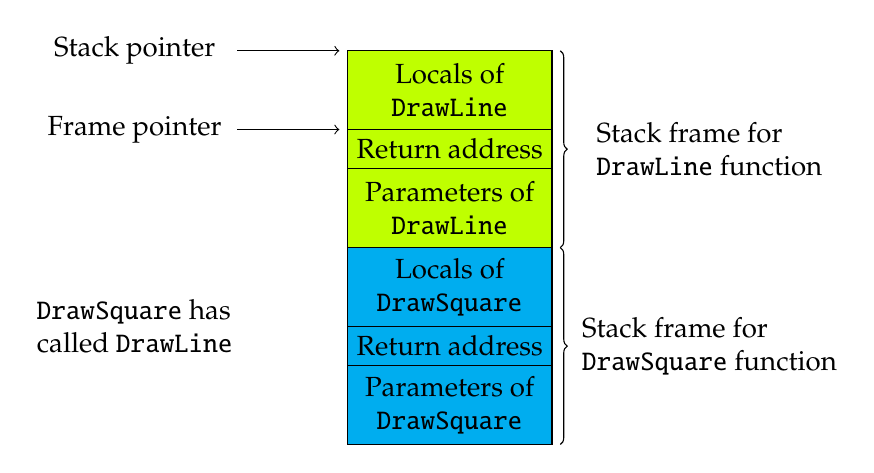
\begin{tikzpicture}

\node[align=left] at (-4,1) {Stack pointer};
\draw[->] (-2.7,1) -- (-1.4,1);
\node[align=left] at (-4,0) {Frame pointer};
\draw[->] (-2.7,0) -- (-1.4,0);

\node[align=left] at (-4,-2.5) {\texttt{DrawSquare} has\\ called \texttt{DrawLine}};
%Stack frame for\\ \texttt{DrawLine} function
%Stack frame for\\ \texttt{DrawSquare} function

\draw[fill=lime] (-1.3, 0) rectangle (1.3, 1) {};
\node[align=center] at (0,0.5) {Locals of\\\texttt{DrawLine}};
\draw[fill=lime] (-1.3, 0) rectangle (1.3, -0.5) {};
\node[align=center] at (0,-0.25) {Return address};
\draw[fill=lime] (-1.3, -1.5) rectangle (1.3, -0.5) {};
\node[align=center] at (0,-1) {Parameters of\\\texttt{DrawLine}};

\draw[decoration={brace,mirror,raise=3pt},decorate] (1.3,-1.5) -- (1.3,1);
\node[align=left] at (3.3,-0.25) {Stack frame for\\ \texttt{DrawLine} function};

\begin{scope}[shift={(0,-2.5)}]
\draw[fill=cyan] (-1.3, 0) rectangle (1.3, 1) {};
\node[align=center] at (0,0.5) {Locals of\\\texttt{DrawSquare}};
\draw[fill=cyan] (-1.3, 0) rectangle (1.3, -0.5) {};
\node[align=center] at (0,-0.25) {Return address};
\draw[fill=cyan] (-1.3, -1.5) rectangle (1.3, -0.5) {};
\node[align=center] at (0,-1) {Parameters of\\\texttt{DrawSquare}};

\draw[decoration={brace,mirror,raise=3pt},decorate] (1.3,-1.5) -- (1.3,1);
\node[align=left] at (3.3,-0.25) {Stack frame for\\ \texttt{DrawSquare} function};
\end{scope}
\end{tikzpicture}



\section{Code block scope}
\begin{itemize}
\item Block scope refers to any code block not just functions
\begin{minted}{c}
if (a > b) {
  int tmp = a;
  // tmp is local to this code block

  a = b;
  b = tmp;
}
\end{minted}
\item \verb!tmp! is automatic and local
\end{itemize}



\section{Static and global variables}
\begin{itemize}
\item \verb!static! variables exist for the duration of the program
\item Variables declared outside a function are visible to all code in the same program and are \verb!static! by default
\begin{minted}{c}
// scope inside a single source file
int a = 10;       // global & static
static int c = 1; // file & static

foo(){
  int tmp = 3;    // local automatic
  static int count = 0; // local static
  a = a + tmp;
  count++;
}
\end{minted}

\item Same \verb!count! variable each time you call \verb!foo()!
\end{itemize}



\section{Function parameters}
\begin{itemize}
\item Parameters have the same properties as local variables
\begin{itemize}
\item i.e. automatic storage duration and block scope
\item Each formal parameter is initialized automatically when a function is called (by being assigned the actual value of the corresponding argument)
\end{itemize}
\end{itemize}



\section{Summary of scope in a single file}
\begin{itemize}
\item \verb!file1.c!:
\end{itemize}
\begin{minted}{c}
int gv;               // gv - global scope (static)

static int fv;        // fv - file scope (static)

void f( int pv ){     // pv - block scope of f()
                      //    (automatic)

   int lv = 0;        // lv - block scope (automatic)

   static int sv = 0; // sv - blck scope (static)
}
\end{minted}



\section{Pros and cons of global variables}
\begin{itemize}
\item Global variables are convenient when many functions must share a variable or when a few functions share a large number of variables
\item In most cases, it's better for functions to communicate through parameters rather than shared variables:
\begin{itemize}
\item If we change a global variable during program maintenance (by altering its type, say), we'll need to check every function in the same file to see how the change affects it
\item If a global variable is assigned an incorrect value, it may be difficult to identify the guilty function
\item Functions that rely on global variables are hard to reuse in other programs
\end{itemize}
\end{itemize}


\end{document}
